%%%%%%%%%%%%%%%%%%%%%%%%%%%%%%%%%%%%%%%%%%%%%%%%%%%%%%%%%%%%%%%%%%%%
% Informe técnico y análisis de resultados del Proyecto 4, EL-4201 Procesamiento Electrónico de Potencia
% Compilar con make. Los datos que todavía no existen van con \pendiente{...}
%%%%%%%%%%%%%%%%%%%%%%%%%%%%%%%%%%%%%%%%%%%%%%%%%%%%%%%%%%%%%%%%%%%%

\documentclass[journal]{IEEEtran}
% Preámbulo común del documento de diseño y del informe técnico de PEDP
\usepackage{instructivo}
\renewcommand{\IEEEkeywordsname}{Palabras clave}
\usepackage[american,siunitx]{circuitikz}

\sisetup{per-mode=symbol, group-digits=integer, output-decimal-marker={,}}
\graphicspath{{./}{./fig/}}

\usepackage{amsmath}
\usepackage{float}
\usepackage[natbib=true,style=trad-unsrt,backend=biber]{biblatex}
\addbibresource{literatura.bib}
\renewcommand*{\bibfont}{\footnotesize}

% Columnas de tabularx que parten el texto en varias líneas para no salirse de la columna
\newcolumntype{L}{>{\raggedright\arraybackslash}X}
\newcolumntype{C}{>{\centering\arraybackslash}X}

% Marcador visible para datos que todavía no existen, nunca se llena con un valor calculado
\newcommand{\pendiente}[1]{\textcolor{red}{\textbf{[#1]}}}

\hyphenation{op-tical net-works semi-conduc-tor}


\begin{document}
\deactivatequoting
\title{Informe técnico del control de corriente de un inversor monofásico en puente H con regulador PR discreto}

\author{Jefferson~Chinchilla~Q.,~\IEEEmembership{Estudiante,~ITCR,}
	Nicolás~Mena~V.,~\IEEEmembership{Estudiante,~ITCR,}
	y~Mattio~Coghi~Q.,~\IEEEmembership{Estudiante,~ITCR}
}

\markboth{Procesamiento Electrónico de Potencia, IIS2026}%
{Proyecto 4: control de corriente con regulador PR}

\maketitle

\begin{abstract}
	% Números y unidades con el mismo peso que el texto en negrita del resumen
	\sisetup{mode=text, reset-text-series=false, text-series-to-math=true, propagate-math-font=true, reset-math-version=false}
	\boldmath\DeclareSIUnit{\ohm}{\ensuremath{\Omega}}
	Se presentan los ensayos de banco del inversor en puente H con carga de \SI{11.8}{\ohm} y \SI{212}{\micro H}, controlado por un regulador proporcional-resonante en un MicroBlaze V con bus de \SI{18}{V}. El firmware mide el cero del sensor al habilitar con el puente conmutando. Según el sensor de la placa, el regulador lleva la corriente a la referencia con menos de \SI{0.5}{\percent} de error y menos de \ang{0.02} de desfase a \num{0.2}, \num{0.5} y \SI{1.0}{A} pico. El osciloscopio sobre la resistencia de la carga da una corriente física entre \num{2.9} y \SI{4}{\percent} por debajo de la referencia. Con la carga aumentada se cumple a \num{0.2} y \SI{0.5}{A}, y a \SI{1.0}{A} la acción satura porque la carga pide más tensión que la disponible, con \SI{-8.6}{\percent} de error. El rizado medido, de \num{0.275}, \num{0.465} y \SI{0.526}{A} pico a pico, supera el límite de \SI{0.20}{A} como predijeron el análisis y la simulación conmutada. Los escalones de consigna se establecen en unos \SI{30}{ms} y el cambio de carga no se distingue en la corriente. El tiempo muerto medido es de \SI{1}{\micro s} en la pierna B y de \SI{1.23}{\micro s} y \SI{430}{ns} en la pierna A.
\end{abstract}


\begin{IEEEkeywords}
	Controlador proporcional-resonante, inversor en puente H, modulación unipolar, tiempo muerto.
\end{IEEEkeywords}

\section{Introducción}
\label{sec:intro}
\IEEEPARstart{E}{ste} informe reúne los resultados experimentales del componente de potencia del Proyecto 4 \cite{enunciado}, un inversor monofásico en puente H con carga $R$--$L$ y un regulador proporcional-resonante discreto \cite{teodorescu2006} que corre en un MicroBlaze V sobre una Basys~3. Se presentan los parámetros medidos del montaje, el método de adquisición y de procesamiento, los registros de los ensayos, el error de amplitud y el desfase de la fundamental, el rizado de conmutación y la comparación con el análisis y con las simulaciones. El dimensionamiento, el modelo de la planta y el diseño del regulador están en el documento de diseño, y aquí se citan solo los valores que hacen falta para comparar. Los registros crudos y los scripts de procesamiento están en el repositorio del proyecto \cite{repositorio}.

Los criterios del enunciado \cite{enunciado} son un error relativo de amplitud de la fundamental menor a \SI{10}{\percent} en una ventana de al menos cinco períodos de \SI{50}{Hz} para referencias de \num{0.2}, \num{0.5} y \SI{1.0}{A} pico, y un rizado de conmutación menor a \SI{0.20}{A} pico a pico. Además se evalúan los cambios de referencia de \num{0.2} a \num{0.5} y de \num{0.5} a \SI{1.0}{A}, y un cambio de la resistencia de al menos \SI{25}{\percent} con \SI{0.5}{A}. Todos tienen registro en los ensayos finales. Los ensayos preliminares quedan como antecedente en la Sección~\ref{sec:antecedente}, porque lo que se encontró en ellos motivó los cambios del firmware y del acondicionador.

\section{Parámetros medidos del montaje}
\label{sec:caract}
La carga son dos resistencias de \SI{4.7}{\ohm} y \SI{5}{W} en serie con dos inductores de \SI{100}{\micro H}. Las resistencias y la resistencia total con inductores y cables se midieron con multímetro, a dos hilos y en frío, y los inductores con un medidor LCR a \SI{1}{kHz}. La Tabla~\ref{tab:caract} compara lo nominal del documento de diseño con lo medido en banco.

\begin{table}[!ht]
	\centering
	\caption{Caracterización del montaje.}
	\label{tab:caract}
	\begin{tabularx}{\columnwidth}{>{\hsize=1.1\hsize}Lc>{\hsize=0.9\hsize}L}
		\toprule
		Magnitud & Nominal & Medido \\
		\midrule
		$R$ de las resistencias & \SI{9.4}{\ohm} & \SI{9.46}{\ohm} \\
		$R$ total con devanados y cables & --- & \SI{11.8}{\ohm} \\
		$R$ total de la carga aumentada & \SI{14.3}{\ohm} & \SI{15.7}{\ohm}, de la acción \\
		$L$ total & \SI{200}{\micro H} & \SI{212}{\micro H}, \SI{106.2}{\micro H} cada uno \\
		Tiempo muerto, pierna A & \SI{1.00}{\micro s} & \SI{1.23}{\micro s} y \SI{430}{ns} \\
		Tiempo muerto, pierna B & \SI{1.00}{\micro s} & \SI{1.00}{\micro s} en ambos flancos \\
		Período de la rutina (JB1) & \SI{50}{\micro s} & \SI{50}{\micro s} \\
		Cero del sensor & \num{2048} cuentas & medido al habilitar \\
		Bus y límite de la fuente & \SI{18}{V} & \SI{18}{V}, \SI{0.74}{A} \\
		\bottomrule
	\end{tabularx}
\end{table}

La resistencia total de \SI{11.8}{\ohm} queda \SI{2.3}{\ohm} por encima de las resistencias por los devanados, las conexiones y el cableado. Los dos inductores midieron \SI{106.2}{\micro H}, \SI{6}{\percent} sobre su nominal. Para el ensayo de carga se añadieron \SI{2.5}{\ohm} en serie. Con los valores nominales la carga quedaría en \SI{14.3}{\ohm}. Como valor de trabajo se toman los \SI{15.7}{\ohm} que corresponden a la acción de control en banco, frente a los \SI{12.2}{\ohm} que da el mismo método con la carga nominal (Sección~\ref{sec:res_tension}). Es un cambio de \SI{29}{\percent}, por encima del \SI{25}{\percent} del enunciado. El multímetro dio \SI{18.7}{\ohm} a dos hilos, pero esa lectura no es compatible con la acción, que a \SI{0.5}{A} habría tenido que llegar a unos \SI{10.4}{V} y llegó a \SI{8.9}{V}, y no se usa. Lo más probable es que incluya la resistencia de los contactos, aunque no se comprobó. Con \SI{1.0}{A} pico cada resistencia de \SI{4.7}{\ohm} disipa \SI{2.35}{W}, el \SI{47}{\percent} de su nominal, y la de \SI{2.5}{\ohm} \SI{1.25}{W}. No se midieron temperaturas, así que el margen de disipación sale de esa cuenta.

\section{Montaje y adquisición}
\label{sec:montaje}
Cada ensayo se registra por dos caminos. El histórico del controlador se toma por la UART a \num{115200} baudios, una trama de \num{12310} bytes con \num{2048} registros a \SI{20}{kS/s}, es decir \SI{102}{ms} o cinco períodos de \SI{50}{Hz}, con la corriente que ve el sensor ACS712 \cite{acs712}, la referencia, la acción y las banderas de saturación y falla. Un osciloscopio GW Instek mide con una sola punta la tensión sobre la resistencia de \SI{9.6}{\ohm} de la carga, y esa tensión dividida entre \SI{9.6}{\ohm} es la corriente física. Las compuertas se midieron en los ensayos preliminares con el osciloscopio Keysight DSO-X 2002A \cite{dsox2000}, con las puntas contra la tierra de potencia, el bus apagado y los \SI{15}{V} de los drivers puestos.

El firmware de los ensayos mide el cero del sensor al subir \texttt{enable}. Deja el puente conmutando con la acción en cero, descarta \num{256} muestras y promedia las \num{1024} siguientes, unos \SI{64}{ms} en total, y usa ese promedio como cero. La pendiente es $k=-\SI{1.292e-3}{A}$ por cuenta, calibrada contra el osciloscopio con los registros de los ensayos preliminares (Sección~\ref{sec:antecedente}). El amplificador AD822 del acondicionador se alimentó a \SI{10}{V}, porque a \SI{5}{V} su salida se quedaba plana cerca de \SI{0.49}{V} y recortaba el lado positivo de la corriente.

\begin{table}[!ht]
	\centering
	\caption{Archivos de captura de los ensayos finales, con rutas relativas a \texttt{muestras\_Inversor/}.}
	\label{tab:archivos}
	\small
	\begin{tabularx}{\columnwidth}{Lcc}
		\toprule
		Archivo & Muestreo & Ventana \\
		\midrule
		CSV del receptor, \texttt{mediciones\_\allowbreak finales/\allowbreak *.csv} & \SI{50}{\micro s} & \SI{102}{ms} \\
		\texttt{mediciones\_\allowbreak finales/\allowbreak transitorios/\allowbreak escalon\_*} & \SI{20}{\micro s} & \SI{200}{ms} \\
		\texttt{mediciones\_\allowbreak finales/\allowbreak transitorios/\allowbreak cambio\_R\_0.5A} y \texttt{arranque\_0-0.2A} & \SI{5}{\micro s} & \SI{50}{ms} \\
		\texttt{Muestras Osciloscopio/\allowbreak rizado/\allowbreak rizado\_18V\_*.csv} & \SI{20}{ns} & \SI{200}{\micro s} \\
		\texttt{Muestras Compuertas/\allowbreak scope\_a\_\allowbreak piernaB\_\allowbreak tiempo\_\allowbreak muerto\_\allowbreak alta\_\allowbreak apaga.png} y \texttt{scope\_a1\_\allowbreak piernaB\_\allowbreak tiempo\_\allowbreak muerto\_\allowbreak baja\_\allowbreak apaga.png}, preliminares & \SI{1}{ns} & \SI{10}{\micro s} \\
		\texttt{Muestras Compuertas/\allowbreak scope\_a5\_\allowbreak habilitar.png} y \texttt{scope\_a6\_\allowbreak deshabilitar.png}, preliminares & \SI{10}{\micro s} & \SI{500}{\micro s} \\
		\bottomrule
	\end{tabularx}
\end{table}

Las dos fuentes de datos miden la corriente por caminos distintos y por eso se comparan. Una diferencia sistemática entre ambas apunta a la ganancia o al cero del sensor.

\section{Procesamiento y resultados}
\label{sec:resultados}
\subsection{Procesamiento}
\label{sec:proc}
La corriente se muestrea una vez por período de portadora, en el valle, así que el histórico no contiene el rizado de conmutación. Sobre los últimos cinco períodos enteros se ajusta por mínimos cuadrados una senoidal de \SI{50}{Hz} más un término constante, a la corriente y a la referencia, igual que \texttt{potencia/analizar\_csv.m}. El error de amplitud es $|\,|I_1|-|R_1|\,|/|R_1|$ y el desfase es positivo cuando la corriente adelanta. Las capturas del osciloscopio se ajustan igual en ventanas de \SI{20}{ms}. El rizado se mide con \texttt{potencia/analizar\_rizado.py}, que se describe en la Sección~\ref{sec:res_rizado}.

\subsection{Seguimiento de la fundamental}
\label{sec:res_nominal}
La Tabla~\ref{tab:med_nominal} resume los siete registros con el lazo cerrado, y la Fig.~\ref{fig:banco} muestra los seis con corriente.

\begin{table*}[!t]
	\centering
	\caption{Seguimiento según el sensor con \SI{18}{V}, ajuste de cinco períodos. Criterio, error menor a \SI{10}{\percent}.}
	\label{tab:med_nominal}
	\begin{tabularx}{\textwidth}{Lccccccc}
		\toprule
		Registro & Carga & Ref. (A) & Medida (A) & Error (\%) & Desfase (°) & Continua (A) & Saturadas \\
		\midrule
		\texttt{0A} & nominal & 0 & \num{0.0002} & --- & --- & $+0.002$ & 0 \\
		\texttt{0.2A} & nominal & \num{0.1993} & \num{0.2002} & \num{0.42} & $-0.02$ & $+0.010$ & 0 \\
		\texttt{0.5A} & nominal & \num{0.4993} & \num{0.4997} & \num{0.08} & \num{0.02} & $-0.003$ & 0 \\
		\texttt{1.0A} & nominal & \num{0.9994} & \num{1.0001} & \num{0.07} & \num{0.01} & $+0.010$ & 0 \\
		\texttt{carga25\_0.2A} & aumentada & \num{0.1994} & \num{0.2000} & \num{0.33} & $-0.01$ & $+0.015$ & 0 \\
		\texttt{carga25\_0.5A} & aumentada & \num{0.4993} & \num{0.5002} & \num{0.17} & \num{0.00} & $+0.008$ & 0 \\
		\texttt{carga25\_1.0A} & aumentada & \num{0.9994} & \num{0.9132} & $-8.62$ & \num{13.91} & $+0.020$ & 20 \\
		\bottomrule
	\end{tabularx}
\end{table*}

\begin{figure*}[!t]
	\centering
	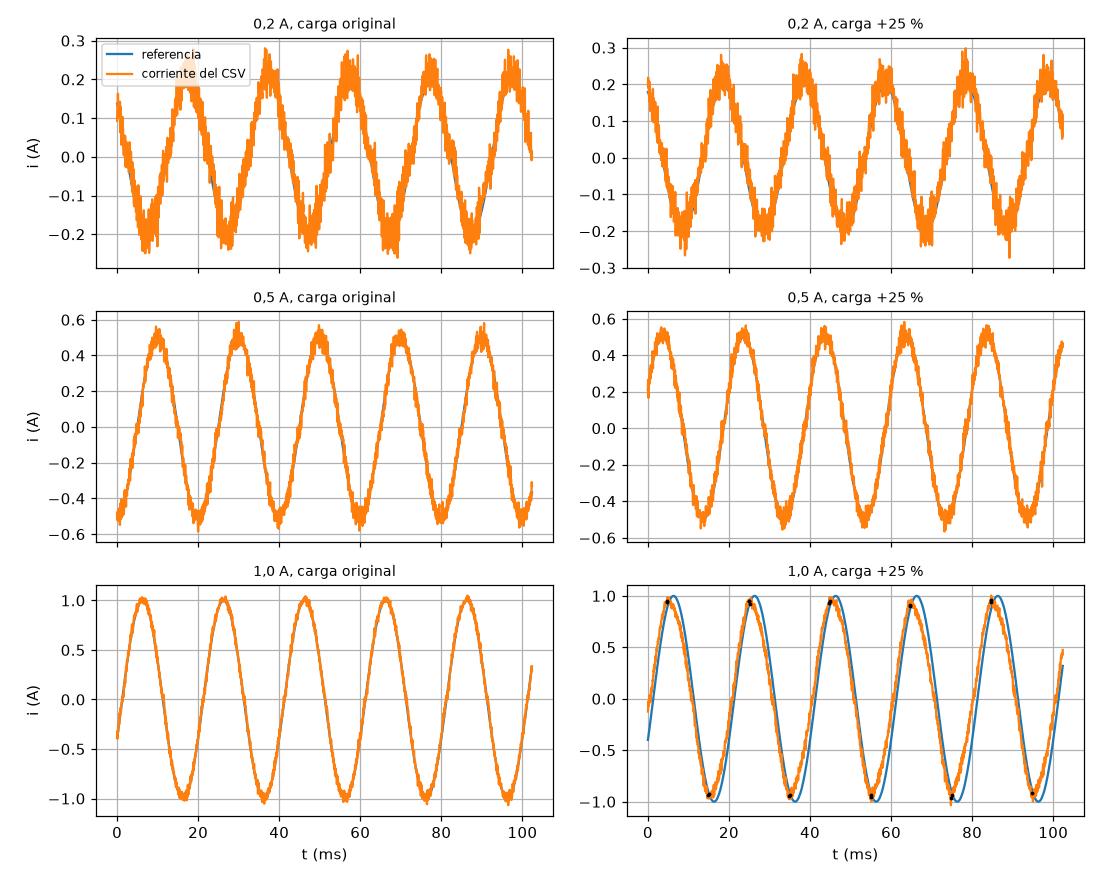
\includegraphics[width=0.85\textwidth]{banco_regimen}
	\caption{Corriente según el sensor y referencia en seis registros de \SI{102}{ms} con \SI{18}{V}, carga nominal a la izquierda y aumentada a la derecha. Los puntos negros marcan las muestras con la acción saturada.}
	\label{fig:banco}
\end{figure*}

Con la carga nominal el resonante lleva el error por debajo de \SI{0.5}{\percent} con desfase nulo en los tres puntos, que es lo esperable de un PR con ganancia infinita en \SI{50}{Hz} \cite{teodorescu2006,yepes2010}. Con la carga aumentada pasa lo mismo a \num{0.2} y \SI{0.5}{A}. La continua queda dentro de $\pm\SI{0.02}{A}$ en todos los registros, contra \num{0.12} a \SI{0.33}{A} con el cero fijo de los ensayos anteriores.

A \SI{1.0}{A} con la carga aumentada la acción llega a $\pm\num{0.92}$ en 20 muestras, 11 en el semiciclo positivo y 9 en el negativo, y los picos instantáneos llegan a $+\num{1.00}$ y $-\SI{1.03}{A}$. La saturación aplana la senoide alrededor de cada pico, la fundamental queda en \SI{0.913}{A} y el desfase sube a \ang{14}. El error cumple el \SI{10}{\percent} por poco. La Sección~\ref{sec:saturacion} explica por qué satura.

\subsection{Corriente física frente al osciloscopio}
\label{sec:res_ganancia}
La Tabla~\ref{tab:ganancia} compara la fundamental del sensor con la del osciloscopio en los tramos estables de las capturas de los transitorios. Las capturas no son del mismo minuto que los CSV, pero sí de la misma sesión, con el mismo firmware y el mismo montaje.

\begin{table}[!ht]
	\centering
	\caption{Fundamental según el sensor y según el osciloscopio, \SI{18}{V}. $^{*}$Carga aumentada.}
	\label{tab:ganancia}
	\begin{tabularx}{\columnwidth}{cCCc}
		\toprule
		Ref. (A) & Sensor (A) & Osc. (A) & Error físico (\%) \\
		\midrule
		\num{0.2} & \num{0.2002} & \num{0.192} & $-3.9$ \\
		\num{0.5} & \num{0.4997} & \num{0.48} & $-4$ \\
		\num{1.0} & \num{1.0001} & \num{0.971} & $-2.9$ \\
		\num{0.5}$^{*}$ & \num{0.5002} & \num{0.477} & $-4.5$ \\
		\bottomrule
	\end{tabularx}
\end{table}

La corriente física queda dentro del \SI{10}{\percent} en los tres puntos, así que el criterio se cumple también con una medición independiente del sensor. Las referencias son amplitudes pico, con valores RMS de \num{0.141}, \num{0.354} y \SI{0.707}{A}, y las corrientes físicas equivalen a \num{0.136}, \num{0.34} y \SI{0.687}{A} RMS de fundamental. El desfase de la corriente física no se puede obtener de estas capturas, porque el osciloscopio no registró la referencia, así que los desfases del informe son según el sensor.

La corriente física queda por debajo de la referencia, y las simulaciones predecían que quedaría por encima, entre \num{2} y \SI{10}{\percent} sobre la muestra del valle (Sección~\ref{sec:comparacion}). En banco queda unos \SI{4}{\percent} por debajo.

La causa más probable es la pendiente $k$. Se calibró con los ensayos preliminares, cuando el AD822 estaba a \SI{5}{V} y comprimía el lado positivo de la señal, y quedó \SI{16}{\percent} por encima del valor nominal para compensar esa compresión. En esos ensayos el cociente entre osciloscopio y sensor crecía con la amplitud, \num{1.14}, \num{1.19} y \num{1.27}, que es la huella de una compresión. Con el AD822 a \SI{10}{V} la cadena deja de comprimir y entrega más cuentas por amperio, pero el firmware siguió con la pendiente anterior. El firmware estima entonces más corriente de la que hay, y el regulador baja la corriente real hasta que la estimación coincide con la referencia. Si el acondicionador no hubiera cambiado, con la pendiente calibrada el osciloscopio habría dado unos \num{1.02} veces la referencia a \SI{0.5}{A} y \num{0.98} a \SI{0.2}{A}, los cocientes preliminares divididos entre \num{1.162}. Dio \num{0.96} en los dos puntos, así que la ganancia de la cadena subió entre \num{2} y \SI{6}{\percent}, más a mayor amplitud, como corresponde a una compresión que desaparece.

La causa no se confirmó con una medición directa. Pueden sumar o restar unos puntos la resistencia donde va la punta, que se toma como \SI{9.6}{\ohm} cuando antes se registraron \SI{9.46}{\ohm}, la exactitud vertical del osciloscopio y la alimentación del ACS712, cuya sensibilidad es proporcional a $V_{CC}$ \cite{acs712}. Recalibrar la pendiente con los datos actuales, unos $-\SI{1.24e-3}{A}$ por cuenta, dejaría la corriente física centrada en la referencia.

\subsection{Tensión aplicada a la carga}
\label{sec:res_tension}
El bus no se registró durante las capturas. Como estimación, la fundamental del índice de modulación del histórico por \SI{18}{V} da la tensión que pidió el regulador (Tabla~\ref{tab:tension}), sin el tiempo muerto ni las caídas en los MOSFET. En el registro saturado el índice recortado no es senoidal y la tabla da solo su fundamental.

\begin{table}[!ht]
	\centering
	\caption{Fundamental del índice de modulación $m_1$ y tensión estimada $V_1=m_1V_{dc}$ con \SI{18}{V}, en valores pico.}
	\label{tab:tension}
	\begin{tabularx}{\columnwidth}{cCcc}
		\toprule
		Ref. (A) & Carga & $m_1$ & $V_1$ (V) \\
		\midrule
		\num{0.2} & nominal & \num{0.172} & \num{3.09} \\
		\num{0.5} & nominal & \num{0.368} & \num{6.63} \\
		\num{1.0} & nominal & \num{0.714} & \num{12.85} \\
		\num{0.2} & aumentada & \num{0.233} & \num{4.19} \\
		\num{0.5} & aumentada & \num{0.495} & \num{8.90} \\
		\num{1.0} & aumentada & \num{0.860} & \num{15.49} \\
		\bottomrule
	\end{tabularx}
\end{table}

Con la carga nominal, la recta entre los puntos de \num{0.2} y \SI{1.0}{A} con la corriente del sensor tiene una pendiente de \SI{12.2}{\ohm} y una ordenada de \SI{0.65}{V}. La pendiente queda cerca de los \SI{11.8}{\ohm} de la carga más unos \SI{0.4}{\ohm} de los dos MOSFET en conducción. La ordenada corresponde a la pérdida por tiempo muerto, una onda cuadrada de $2t_df_{sw}V_{dc}=\SI{0.72}{V}$ en fase con la corriente \cite[sec.~8-5]{mohan2003power}, cuya fundamental vale \SI{0.92}{V}. Con la carga aumentada, la recta entre \num{0.2} y \SI{0.5}{A} da \SI{15.7}{\ohm} y \SI{1.05}{V}.

A \SI{0.5}{A} la corriente queda igual con las dos cargas y el índice sube de \num{0.368} a \num{0.495}, \num{1.34} veces. El regulador compensó el cambio de carga subiendo la tensión aplicada, que es lo que se espera del ensayo en régimen. Con las rectas de las dos cargas la resistencia pasa de \num{12.2} a \SI{15.7}{\ohm}, un \SI{29}{\percent} más, que es el cambio que se reporta para el ensayo.

\subsection{Transitorios}
\label{sec:res_transitorios}
Los transitorios se registraron con el osciloscopio sobre la resistencia de la carga. La referencia no da escalones, porque el firmware limita su cambio a \SI{1}{A} cada \SI{20}{ms}.

En el escalón de \num{0.5} a \SI{1.0}{A} (Fig.~\ref{fig:transitorios}) la fundamental pasa de \num{0.485} a \SI{0.97}{A} y se establece en unos \SI{30}{ms}, la rampa más un poco de respuesta del regulador, sin oscilación visible. En el de \num{0.2} a \SI{0.5}{A} la corriente pasa unos \SI{30}{ms} por cero. La amplitud se elige con dos interruptores, donde 01 es \SI{0.2}{A} y 10 es \SI{0.5}{A}, y al bajar el primero antes de subir el segundo se pasa por 00, que es \SI{0}{A}. Desde cero llega a \SI{0.48}{A} en unos \SI{30}{ms}.

En el cambio de resistencia a \SI{0.5}{A} la fundamental queda en \SI{0.48}{A} en toda la ventana de \SI{50}{ms}, sin transitorio visible a esa escala. Para el regulador el cambio de carga es una perturbación de \SI{50}{Hz}, que el resonante rechaza \cite{teodorescu2006}. Que la carga cambió se ve en la acción de la Sección~\ref{sec:res_tension}.

\begin{figure}[!ht]
	\centering
	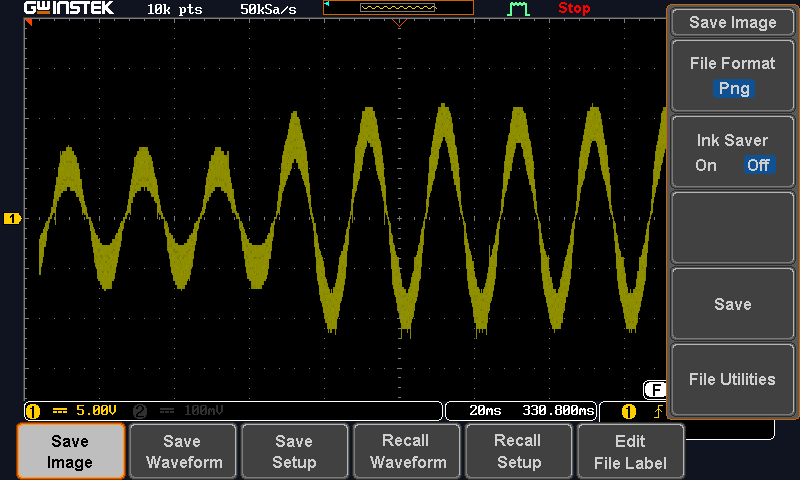
\includegraphics[width=\columnwidth]{transitorio_escalon_05_10}\\[2pt]
	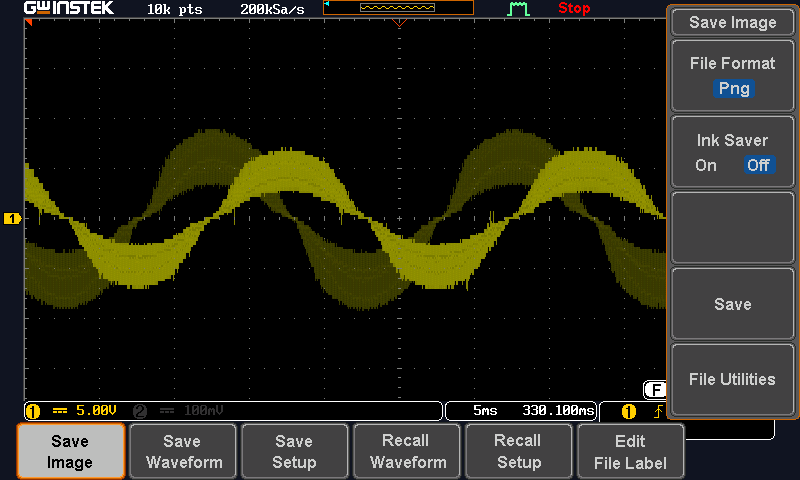
\includegraphics[width=\columnwidth]{transitorio_cambio_r}
	\caption{Tensión sobre la resistencia de \SI{9.6}{\ohm}, \SI{5}{V/div}. Arriba, escalón de consigna de \num{0.5} a \SI{1.0}{A}, \SI{20}{ms/div}. Abajo, cambio de carga a \SI{0.5}{A}, \SI{5}{ms/div}, con dos barridos superpuestos.}
	\label{fig:transitorios}
\end{figure}

\subsection{Compuertas y tiempo muerto}
\label{sec:res_compuertas}
En una primera prueba con el bus apagado se midió \SI{1}{\micro s} de tiempo muerto en los cuatro flancos a \num{10}, \num{20} y \SI{40}{kHz}, los \SI{70}{\micro s} de precarga con las dos bajas encendidas, y se vio que al apagar el último pulso del alto sale recortado a unos \SI{20}{\micro s} porque el núcleo apaga en el valle, donde el alto está centrado. En los ensayos preliminares se repitió con la placa actual. La pierna B dio \SI{1}{\micro s} en los dos flancos (Fig.~\ref{fig:tm}). La pierna A dio \SI{1.23}{\micro s} cuando la baja apaga y la alta enciende y \SI{430}{ns} en el otro flanco, según lo anotado en el banco. La captura de esa pierna no está archivada en el repositorio, solo las de la pierna B. Los \SI{430}{ns} quedan bajo el valor programado pero siguen siendo un intervalo sin conducción simultánea, más largo que los tiempos de conmutación del IRF520N \cite{irf520n}. La asimetría sale de los retardos distintos de encendido y apagado del VO3120 y del IR2110 de esa pierna \cite{vo3120,ir2110}. Como la pérdida de tensión es proporcional al tiempo muerto \cite[sec.~8-5]{mohan2003power}, la pierna A pierde algo menos que lo que supone el diseño.

\begin{figure}[!ht]
	\centering
	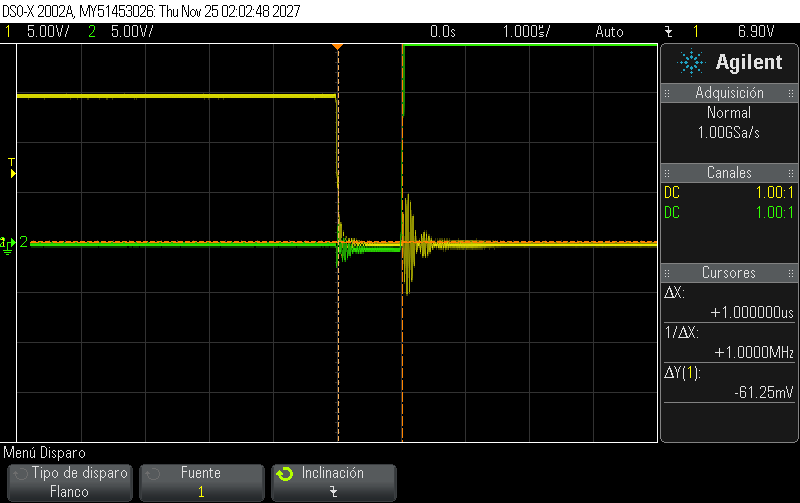
\includegraphics[width=\columnwidth]{tiempo_muerto}
	\caption{Tiempo muerto de \SI{1}{\micro s} entre el apagado de la compuerta alta (CH1) y el encendido de la baja (CH2), \SI{5}{V/div} y \SI{1}{\micro s/div}.}
	\label{fig:tm}
\end{figure}

El pin JB1, que sube al entrar a la rutina periódica y baja al salir, se repite cada \SI{50}{\micro s}. No se midieron la duración ni el jitter de la rutina.

\subsection{Rizado}
\label{sec:res_rizado}
Las capturas se tomaron a \SI{20}{\micro s/div} y \SI{50}{MS/s}, unas \num{1250} muestras por período de \SI{25}{\micro s}, con una sola punta sobre la resistencia. En cada flanco del puente aparecen picos de hasta \SI{3.2}{V} que duran menos de \SI{1}{\micro s}. La corriente por la bobina no puede saltar así, así que son de la medición, probablemente el $dv/dt$ del puente acoplado en la punta y su cable de tierra, y se quitan con una mediana móvil de \SI{1}{\micro s}. La baja frecuencia sale de un promedio móvil de \SI{50}{\micro s}, un período de la portadora, que cancela el rizado al doble de esa frecuencia. El rizado es el pico a pico de lo que queda (Fig.~\ref{fig:rizado}).

\begin{table}[!ht]
	\centering
	\caption{Rizado con \SI{18}{V}. $i_{bf}$ es la corriente de baja frecuencia en la captura y la última columna el modelo de Octave con \SI{9}{\ohm} y \SI{200}{\micro H}.}
	\label{tab:rizado}
	\begin{tabularx}{\columnwidth}{cCcc}
		\toprule
		Ref. (A) & $i_{bf}$ (A) & Rizado (A pp) & Octave (A pp) \\
		\midrule
		\num{0.2} & \num{0.18} & \num{0.275} & \num{0.268} \\
		\num{0.2} & \num{0.09} & \num{0.176} & --- \\
		\num{0.5} & $-0.42$ & \num{0.465} & \num{0.483} \\
		\num{1.0} & $-0.66$ & \num{0.526} & \num{0.597} \\
		\num{1.0} & $-0.21$ & \num{0.294} & --- \\
		\bottomrule
	\end{tabularx}
\end{table}

En la modulación unipolar el rizado crece con $|m|$ hasta \num{0.5} \cite[sec.~8-3-2]{mohan2003power}, así que en cada punto se reporta la captura más cercana al máximo de $|m|$, \num{0.275}, \num{0.465} y \SI{0.526}{A} pico a pico. Las tres superan los \SI{0.20}{A}. Con el nivel de baja frecuencia el índice instantáneo es $m\approx Ri/V_{dc}$, y $\Delta I=V_{dc}\,m(1-m)/(2Lf_{sw})$ con \SI{18}{V} y \SI{212}{\micro H} da \num{0.22}, \num{0.43} y \SI{0.52}{A} en el punto de cada captura principal.

\begin{figure}[!ht]
	\centering
	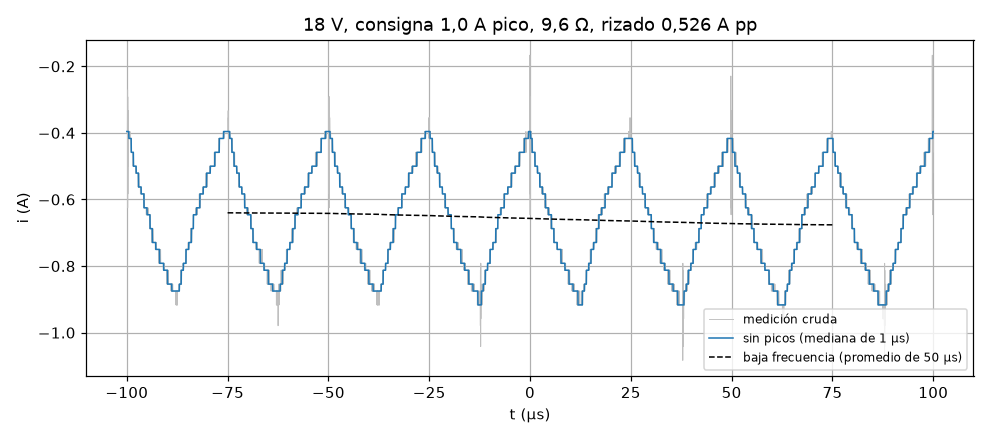
\includegraphics[width=\columnwidth]{rizado_18V_10A}
	\caption{Rizado a \SI{18}{V} y \SI{1.0}{A} pico sobre \SI{9.6}{\ohm}. En gris la medición cruda, en azul sin los picos de conmutación y en negro la baja frecuencia.}
	\label{fig:rizado}
\end{figure}

\subsection{Antecedente de los ensayos preliminares}
\label{sec:antecedente}
Esos ensayos se hicieron con el cero del sensor fijo en \num{2808} cuentas, con \SI{12.5}{V} y \SI{0.52}{A} de límite salvo un punto de \SI{1.0}{A} con \SI{18}{V}, y con el rizado medido restando dos puntas. Esos registros no forman parte de la evidencia de este informe y quedan en el repositorio del proyecto \cite{repositorio}. Con el control deshabilitado el sensor marcaba entre $-\num{0.54}$ y $-\SI{0.65}{A}$ y con el lazo cerrado y referencia nula $+\SI{0.24}{A}$, unas \num{800} cuentas de diferencia entre los dos estados del puente, y el proporcional convertía ese error en una continua física. La corriente física medida con el osciloscopio quedaba \num{14.6} y \SI{18.7}{\percent} sobre la referencia a \num{0.2} y \SI{0.5}{A}. Con esos pares se calibró la pendiente $k$ que usa el firmware actual. El punto de \SI{1.0}{A} se recortaba, con \SI{35}{\percent} de error a \SI{12.5}{V} y \SI{12}{\percent} a \SI{18}{V}, y en banco se vio que el AD822 a \SI{5}{V} aplanaba el lado positivo de la salida del acondicionador. De ahí salieron el autocero y la alimentación del AD822 a \SI{10}{V}.

\section{Simulación en PLECS}
\label{sec:plecs_res}
El modelo del inversor se armó en PLECS 5.0 (Fig.~\ref{fig:plecs}). Tiene el puente con cuatro MOSFET con diodo en antiparalelo y resistencia de conducción $R_{DS(on)}$, la carga $RL$ entre los puntos medios de las piernas, y un modulador unipolar con la referencia retenida en los valles de la portadora y el tiempo muerto armado con dos portadoras corridas $\pm2f_{sw}T_M$. Todos los parámetros salen de \texttt{potencia/sim/parametros.m}, y los ensayos se corren por la interfaz RPC de PLECS desde \texttt{potencia/sim/lazo\_abierto.py}. El documento de diseño describe el modelo completo y su validación contra el análisis.

\begin{figure}[!ht]
	\centering
	\IfFileExists{fig/plecs_modelo.png}{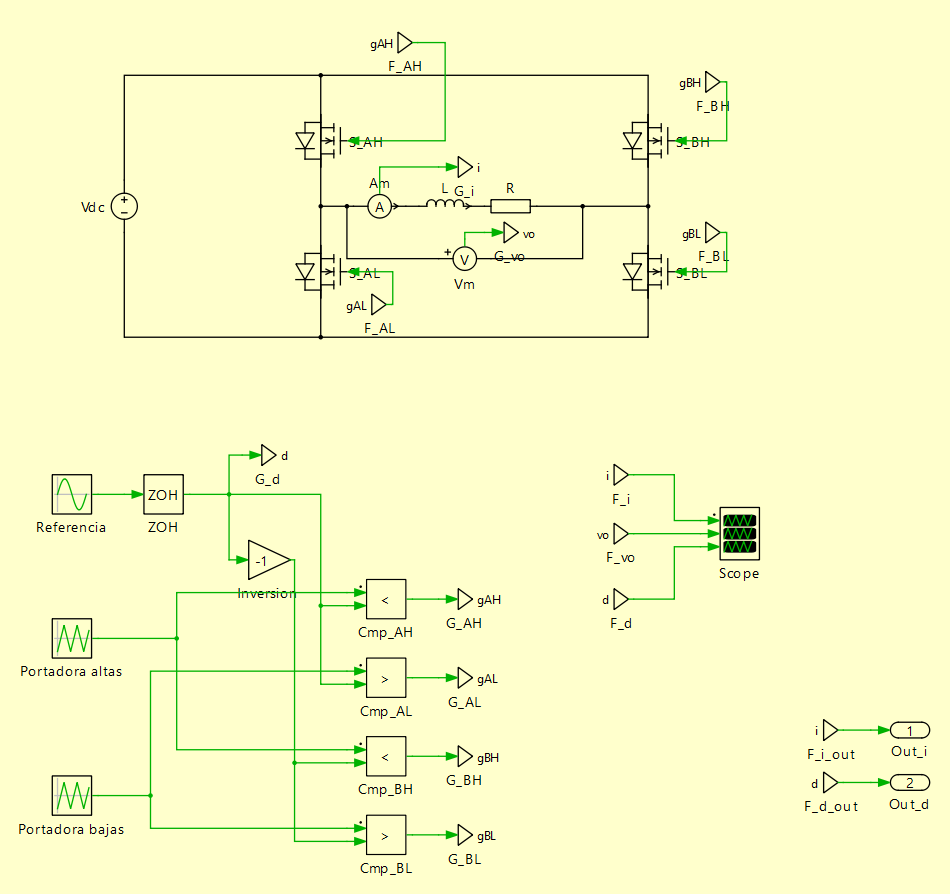
\includegraphics[width=\columnwidth]{plecs_modelo}}{\pendiente{captura del esquema de PLECS en fig/plecs\_modelo.png}}
	\caption{Modelo del inversor en PLECS. Arriba, el puente con la carga $RL$ y los medidores de corriente y tensión. Abajo, la referencia retenida en los valles, las dos portadoras corridas para el tiempo muerto y los cuatro comparadores de las compuertas.}
	\label{fig:plecs}
\end{figure}

Con la carga de diseño se corrió en lazo abierto, con \SI{12}{V}, $R=\SI{9.6}{\ohm}$, $L=\SI{200}{\micro H}$, tiempo muerto de \SI{1}{\micro s} y $R_{DS(on)}=\SI{0.2}{\ohm}$, aplicando el índice $m=|Z|I/V_{dc}$ sin compensar (Tabla~\ref{tab:plecs_abierto}). La corriente queda \num{34}, \num{16} y \SI{10}{\percent} por debajo de lo pedido, con un desfase de $-\ang{0.36}$, y esa diferencia es la que tiene que compensar el regulador. PLECS no se volvió a correr con la carga medida. El modelo analítico de \texttt{potencia/verificar\_pr.m}, que reproduce esta tabla con \SI{9.6}{\ohm} (\num{0.131}, \num{0.419} y \SI{0.899}{A}), da con \SI{11.8}{\ohm}, \SI{212}{\micro H} y \SI{12.5}{V} unas corrientes de \num{0.141}, \num{0.431} y \SI{0.915}{A}, \num{29}, \num{14} y \SI{8}{\percent} por debajo de lo pedido.

\begin{table}[!ht]
	\centering
	\caption{Lazo abierto en PLECS con la carga de diseño, \SI{9.6}{\ohm} y \SI{200}{\micro H}, y \SI{12}{V}.}
	\label{tab:plecs_abierto}
	\begin{tabular}{cccc}
		\toprule
		Pedida (A) & $m$ & Corriente (A) & Diferencia (\%) \\
		\midrule
		\num{0.2} & \num{0.160} & \num{0.1315} & $-34$ \\
		\num{0.5} & \num{0.400} & \num{0.4190} & $-16$ \\
		\num{1.0} & \num{0.800} & \num{0.8989} & $-10$ \\
		\bottomrule
	\end{tabular}
\end{table}

Para el lazo cerrado (Fig.~\ref{fig:plecs_cerrado}) se agregó al mismo modelo el regulador del firmware en un bloque C-Script (\texttt{potencia/sim/lazo\_cerrado.plecs}). El bloque muestrea la corriente en cada valle, aplica los coeficientes de \texttt{sw/pr\_params.h} con la saturación en $\pm\num{0.92}$ y el mismo anti-windup del firmware, y entrega el índice al modulador una muestra después, igual que el periférico, que lo carga en el valle siguiente. La carga es la medida en banco, \SI{11.8}{\ohm} y \SI{200}{\micro H}, y el sensor se toma ideal, sin filtro ni error de ganancia. Los ensayos se corren con \texttt{potencia/sim/lazo\_cerrado.py}, que ajusta la fundamental en los últimos cinco períodos de \SI{0.2}{s} simulados (Tabla~\ref{tab:plecs_cerrado}).

Con un sensor perfecto, la corriente física queda entre \num{6} y \SI{10}{\percent} sobre la referencia, porque el regulador lleva a la referencia la muestra del valle y no el promedio del período. A \SI{1.0}{A} con \SI{12.5}{V} la acción satura, y la corriente queda \SI{8.9}{\percent} por debajo, con \ang{11.5} de desfase. Con \SI{18}{V} el mismo punto no satura, con un índice máximo de \num{0.78}, y tampoco satura con los \SI{2.5}{\ohm} añadidos, donde llega a \num{0.91}. El rizado simulado va de \num{0.28} a \SI{0.56}{A} pico a pico.

\begin{table}[!ht]
	\centering
	\caption{Lazo cerrado en PLECS con el PR del firmware, $L=\SI{200}{\micro H}$ y sensor ideal. $|I_1|$ es la amplitud pico de la fundamental de la corriente física.}
	\label{tab:plecs_cerrado}
	\resizebox{\columnwidth}{!}{%
	\begin{tabular}{cccccccc}
		\toprule
		$I_{ref}$ (A) & $V_{dc}$ (V) & $R$ (\si{\ohm}) & $|I_1|$ (A) & Error (\%) & Desfase & $|m|_{max}$ & Rizado (A pp) \\
		\midrule
		\num{0.2} & \num{12.5} & \num{11.8} & \num{0.2192} & $+9.59$ & \ang{0.20} & \num{0.262} & \num{0.280} \\
		\num{0.5} & \num{12.5} & \num{11.8} & \num{0.5388} & $+7.75$ & \ang{0.19} & \num{0.573} & \num{0.384} \\
		\num{1.0} & \num{12.5} & \num{11.8} & \num{0.9113} & $-8.87$ & \ang{11.50} & \num{0.920} & \num{0.396} \\
		\num{1.0} & \num{18} & \num{11.8} & \num{1.0593} & $+5.93$ & \ang{0.17} & \num{0.776} & \num{0.560} \\
		\num{0.5} & \num{12.5} & \num{14.3} & \num{0.5485} & $+9.71$ & \ang{0.20} & \num{0.691} & \num{0.381} \\
		\num{1.0} & \num{18} & \num{14.3} & \num{1.0604} & $+6.04$ & \ang{0.16} & \num{0.913} & \num{0.555} \\
		\bottomrule
	\end{tabular}}
\end{table}

\begin{figure}[!ht]
	\centering
	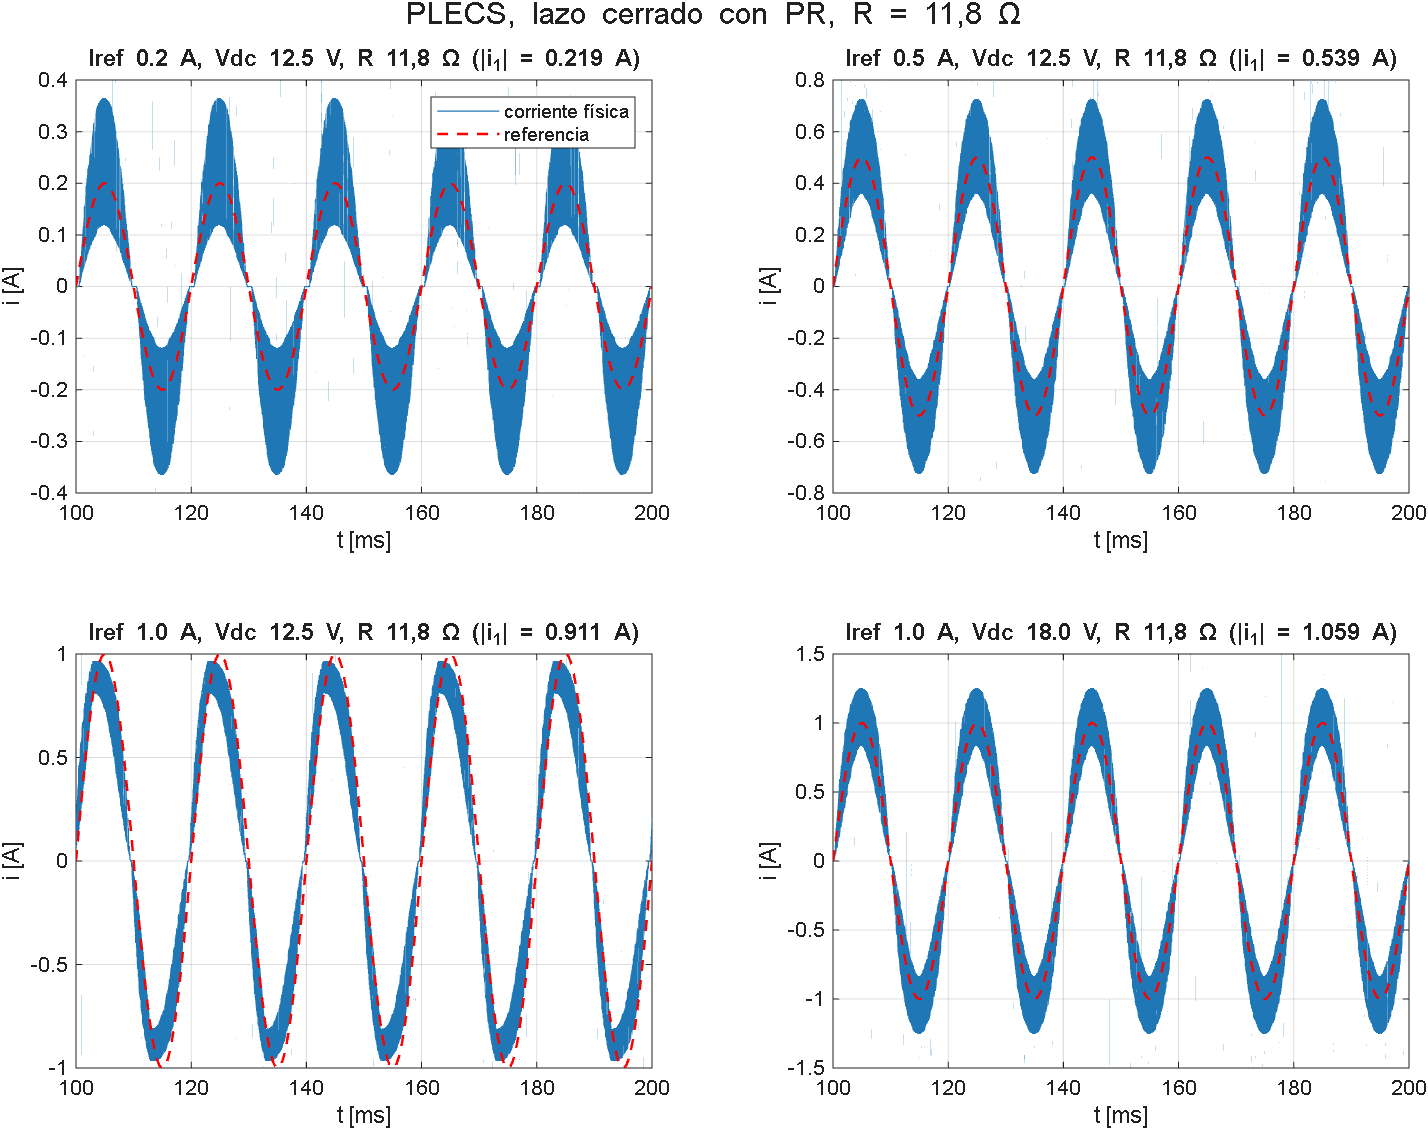
\includegraphics[width=\columnwidth]{plecs_lazo_cerrado}
	\caption{Corriente física y referencia en el lazo cerrado de PLECS, con $R=\SI{11.8}{\ohm}$ y $L=\SI{200}{\micro H}$, en los últimos cinco períodos de la fundamental. Arriba, \num{0.2} y \SI{0.5}{A} con \SI{12.5}{V}. Abajo, \SI{1.0}{A} con \SI{12.5}{V}, donde la acción satura, y con \SI{18}{V}.}
	\label{fig:plecs_cerrado}
\end{figure}

La simulación usa los \SI{200}{\micro H} nominales. Con los dos inductores medidos la total es un \SI{6}{\percent} mayor, lo que baja el rizado en una proporción parecida y reduce un poco el sesgo del valle, que depende de $\tau=L/R$.


\section{Comparación entre teoría, simulación y experimento}
\label{sec:comparacion}
La Tabla~\ref{tab:cmp} pone en una fila cada magnitud con su valor de análisis, de simulación y medido. El análisis son las ecuaciones del documento de diseño evaluadas con la carga medida (\texttt{potencia/verificar\_pr.m} y la fórmula del rizado unipolar). La simulación conmutada es el modelo de Octave \texttt{potencia/simular\_conmutado.m} con los coeficientes del firmware, y la última columna de simulación es el lazo cerrado de PLECS con \SI{11.8}{\ohm} y \SI{200}{\micro H}. Las mediciones son con \SI{18}{V}, y las simulaciones de error físico disponibles con la carga medida son con \SI{12.5}{V}. El sesgo del valle no tiene una forma cerrada simple. Con $\tau=L/R=\SI{18}{\micro s}$, comparable con el período de \SI{50}{\micro s}, los tramos de corriente son exponenciales y la muestra del valle deja de coincidir con el promedio del período, como pasaría con tramos rectos, así que solo las simulaciones lo estiman.

\begin{table*}[!t]
	\centering
	\caption{Comparación por magnitud. Mediciones con \SI{18}{V}.}
	\label{tab:cmp}
	\resizebox{\textwidth}{!}{%
	\begin{tabular}{lcccc}
		\toprule
		Magnitud & Análisis & Simulación conmutada & PLECS lazo cerrado & Medición \\
		\midrule
		Error según el sensor, 0,2 / 0,5 / 1,0 A & \SI{0}{\percent} (resonante ideal) & \SI{0.00}{\percent} & --- & \num{0.42} / \num{0.08} / \SI{0.07}{\percent} \\
		Error de la corriente física, 0,2 / 0,5 A & sesgo del valle, sin forma cerrada & \num{4.94} / \SI{3.79}{\percent} (\SI{12.5}{V}) & \num{9.59} / \SI{7.75}{\percent} (\SI{12.5}{V}) & $-\num{3.9}$ / $-\SI{4}{\percent}$ (osciloscopio) \\
		Error de la corriente física, 1,0 A & --- & \SI{2.4}{\percent} & \SI{5.9}{\percent} & $-\SI{2.9}{\percent}$ \\
		Saturación a \SI{1.0}{A}, carga nominal & no satura, $m=\num{0.73}$ & no satura & no satura, $|m|_{max}=\num{0.78}$ & no satura, $m_1=\num{0.71}$ \\
		Saturación a \SI{1.0}{A}, carga aumentada & al límite, pide \SI{16.7}{V} con \SI{15.7}{\ohm} & --- & no satura con \SI{14.3}{\ohm}, $|m|_{max}=\num{0.91}$ & satura, $-\SI{8.6}{\percent}$ sensor \\
		Cambio de carga a \SI{0.5}{A}, sensor & \SI{0}{\percent} & \SI{0.00}{\percent} (física \SI{5.1}{\percent}) & \SI{9.71}{\percent} (física, \SI{12.5}{V}) & \SI{0.17}{\percent}, física $-\SI{4.5}{\percent}$ \\
		Rizado, 0,2 / 0,5 / 1,0 A (A pp) & \num{0.22} / \num{0.43} / \num{0.52} & \num{0.268} / \num{0.483} / \num{0.597} (\SI{9}{\ohm}) & \num{0.560} a \SI{1.0}{A} & \num{0.275} / \num{0.465} / \num{0.526} \\
		Tiempo muerto & \SI{1.00}{\micro s} & \SI{1.00}{\micro s} (RTL) & --- & B \SI{1.00}{\micro s}, A \SI{1.23}{\micro s} y \SI{430}{ns} \\
		Período de la rutina & \SI{50}{\micro s} & \SI{50}{\micro s} (RTL) & --- & \SI{50}{\micro s} \\
		\bottomrule
	\end{tabular}}
\end{table*}

Lo que coincide es todo lo que depende del lazo visto desde el sensor y la etapa de potencia. El error según el sensor es casi nulo como predicen el análisis y la simulación, el tiempo muerto y el período de la rutina son los programados, y el rizado medido queda a \num{3}, \num{4} y \SI{12}{\percent} de la simulación conmutada. Con la carga nominal y \SI{18}{V}, \SI{1.0}{A} no satura, como predecían el análisis y PLECS. Lo que no coincide es la posición de la corriente física respecto de la referencia. Las dos simulaciones ponen la corriente física sobre la muestra del valle, y el banco la pone unos \SI{4}{\percent} por debajo. PLECS tampoco satura con la carga aumentada porque usa \SI{14.3}{\ohm}, menos que lo que indica la acción en banco.

La diferencia entre las dos simulaciones sale de cómo modelan el tiempo muerto. Alrededor del valle conducen las dos altas, la carga ve \SI{0}{V} y la corriente decae con $\tau=L/R$, así que la muestra depende del punto de ese tramo en que cae la conversión. En el núcleo del PWM y en el modelo de Octave la compuerta que entra se enciende $T_M$ después del cruce, el tramo de tensión nula termina $T_M$ más tarde y su centro queda \SI{0.5}{\micro s} después del valle. En PLECS el hueco está centrado en el cruce, el tramo queda centrado en el valle y la muestra cae en su centro, donde la corriente es menor. Con el modelo de Octave, \SI{11.8}{\ohm}, \SI{212}{\micro H} y \SI{12.5}{V}, moviendo solo el instante de muestreo, el error de la corriente física a \num{0.2} y \SI{0.5}{A} es de \num{2.16} y \SI{0.98}{\percent} con la muestra \SI{0.5}{\micro s} antes del valle, \num{4.94} y \SI{3.79}{\percent} en el valle, \num{7.85} y \SI{6.60}{\percent} \SI{0.5}{\micro s} después y \num{10.93} y \SI{9.45}{\percent} \SI{1}{\micro s} después, unos tres puntos por cada \SI{0.5}{\micro s} (\texttt{simular\_conmutado.m} con el corrimiento del muestreo como sexto argumento, salidas con el sufijo \texttt{\_muestra} en \texttt{docs/\allowbreak informe/\allowbreak evidencia/}). El caso de \SI{0.5}{\micro s} después equivale al centrado de PLECS, y lo que falta hasta sus \num{9.59} y \SI{7.75}{\percent} corresponde a su constante de tiempo menor, con \SI{200}{\micro H} y los \SI{0.4}{\ohm} de los MOSFET.

En el banco la cadena de compuertas atrasa además cada flanco entre \num{0.1} y \SI{0.91}{\micro s} respecto de la orden del núcleo, mientras el XADC convierte en el valle, así que la muestra cae antes del centro del tramo y el sesgo real debería quedar por debajo del de PLECS, del orden del de Octave o menor. Eso reduce el sesgo pero no lo vuelve negativo, así que la diferencia con el banco corresponde a la cadena de medida, con la pendiente del sensor calibrada con el acondicionador anterior como causa más probable (Sección~\ref{sec:res_ganancia}).

\section{Discusión}
\label{sec:discusion}
\subsection{Efecto del cambio de carga}
La carga pasó de \SI{30}{mH} a \SI{200}{\micro H} con el regulador ya diseñado. Con \SI{200}{\micro H} la carga es casi resistiva a \SI{50}{Hz}, y eso hizo fácil el seguimiento de la fundamental, que se ve en los errores menores a \SI{0.5}{\percent} según el sensor. El precio fue el rizado. El rizado de la modulación unipolar baja con $L$ y con la frecuencia de conmutación \cite[sec.~8-3-2]{mohan2003power}. A \SI{20}{kHz} la inductancia no alcanza para bajarlo de \SI{0.20}{A} pico a pico con ningún bus del rango, y la medición lo confirma en los tres puntos. Hacía falta al menos \SI{0.56}{mH}, o subir la portadora a \SI{40}{kHz} con \SI{12}{V}.

El cambio de resistencia a \SI{0.5}{A} no se ve en la corriente. El resonante rechaza la perturbación y la acción sube \num{1.34} veces en régimen.

\subsection{Saturación con la carga aumentada}
\label{sec:saturacion}
Con \SI{18}{V} el tope de \num{0.92} da \SI{16.6}{V}. Con la recta de la Sección~\ref{sec:res_tension}, la carga aumentada pide para \SI{1.0}{A} unos $\SI{15.7}{\ohm}\cdot\SI{1}{A}+\SI{1.05}{V}\approx\SI{16.7}{V}$, justo por encima de lo disponible. Por eso la acción toca el límite en cada pico y la fundamental queda en \SI{0.913}{A}, cerca de la corriente máxima alcanzable. La saturación la explica la carga, y no hace falta suponer que la fuente limitó, que era la hipótesis de los ensayos anteriores. Con la carga nominal, \SI{1.0}{A} pide \SI{12.9}{V} y queda margen.

\subsection{Diferencias entre predicción y práctica}
La diferencia más grande es que la corriente física queda por debajo de la referencia, cuando las simulaciones la ponían por encima. Las simulaciones suponen un sensor con ganancia y cero exactos. En banco el cero ya no aporta error, porque el autocero lo mide en las condiciones de operación y la continua quedó en \SI{0.02}{A} o menos, pero la pendiente viene de una calibración con el AD822 a \SI{5}{V}, que comprimía la señal, y no se recalibró al pasarlo a \SI{10}{V}. Un error de ganancia del sensor cambia igual la amplitud medida y la que el lazo cree que tiene, así que el lazo converge a un valor que difiere del físico en esa proporción. Es la causa más probable de los \SI{4}{\percent} (Sección~\ref{sec:res_ganancia}).

La resistencia de la carga aumentada se toma de la acción de control, \SI{15.7}{\ohm}, porque es el valor compatible con la tensión aplicada en los dos puntos sin saturar y con la saturación a \SI{1.0}{A}. Queda por encima de los \SI{14.3}{\ohm} nominales, probablemente por las conexiones de la resistencia añadida.

\subsection{Limitaciones del modelo}
El lazo promedio no tiene rizado, cuantización ni ruido. El modelo conmutado no tiene el filtro del sensor ni los retardos de los drivers, y supone un sensor con ganancia y cero exactos. Las armónicas impares del tiempo muerto \cite[sec.~8-5]{mohan2003power} no las corrige el resonante, que solo actúa en \SI{50}{Hz}, y deforman la corriente en los cruces por cero sin afectar la fundamental.

\subsection{Limitaciones de las mediciones}
Cada limitación dice qué criterio del enunciado deja sin demostrar.
\begin{itemize}
	\item Tiempo muerto de la pierna A. Los \SI{1.23}{\micro s} y los \SI{430}{ns} salen de lo anotado en el banco y no hay captura. Solo la pierna B tiene captura, con \SI{1}{\micro s} en los dos flancos.
	\item Simultaneidad. Las capturas del osciloscopio no son del mismo minuto que los CSV, aunque sí de la misma sesión.
	\item Corriente física por debajo de la referencia. Queda unos \SI{4}{\percent} por debajo, y las simulaciones predecían que quedaría por encima. La causa más probable es la pendiente calibrada con el AD822 a \SI{5}{V}, sin confirmar con una medición directa.
	\item Resistencia de la carga aumentada. Se toma de la acción de control, \SI{15.7}{\ohm}. La lectura de \SI{18.7}{\ohm} del multímetro no se usa y no se repitió a cuatro hilos.
	\item Desfase de la corriente física. El osciloscopio no registró la referencia, así que solo hay desfase según el sensor.
	\item Resistencia. No se midió a cuatro hilos ni en caliente.
	\item Tensión del bus. Se anotó la de la fuente, \SI{18}{V}, pero no se registró durante las capturas.
	\item Rutina de control y falla. Solo se afirma el período de \SI{50}{\micro s}. El ancho máximo y el jitter, la precarga de \SI{70}{\micro s}, el último pulso truncado, la fase entre ADC, temporizador y PWM, el filtro antialias y la prueba de falla no se midieron.
	\item Plataforma digital. La simulación temporizada del periférico PWM pasó su autochequeo sin errores, pero es del periférico solo y sin retardos de entrada y salida. Los retardos de las compuertas salen del banco y no de esa simulación.
\end{itemize}

\section{Conclusiones}
\label{sec:conclusiones}
El regulador PR cumple el criterio de \SI{10}{\percent} a \num{0.2}, \num{0.5} y \SI{1.0}{A} con la carga nominal y \SI{18}{V}, con menos de \SI{0.5}{\percent} de error y desfase nulo según el sensor, y con la corriente física entre \num{2.9} y \SI{4}{\percent} por debajo de la referencia según el osciloscopio. El autocero dejó la continua dentro de \SI{0.02}{A}. Con la carga aumentada se cumple a \num{0.2} y \SI{0.5}{A}. A \SI{1.0}{A} la acción satura porque la carga pide unos \SI{16.7}{V} y el puente da \SI{16.6}{V}, con \SI{-8.6}{\percent} de error y \ang{14} de desfase.

El rizado medido, de \num{0.275}, \num{0.465} y \SI{0.526}{A} pico a pico, no cumple los \SI{0.20}{A}, como predicen el análisis y la simulación conmutada, a \num{3}, \num{4} y \SI{12}{\percent} de esta última. Bajarlo pide más inductancia o más frecuencia de conmutación.

Los escalones de consigna se establecen en unos \SI{30}{ms}, la rampa de la referencia más la respuesta del regulador. El cambio de resistencia a \SI{0.5}{A} no se distingue en la corriente, y la acción subió \num{1.34} veces para compensarlo. El tiempo muerto y el período de la rutina son los de diseño. Quedan sin demostrar el tiempo muerto de la pierna A con captura y el ancho y el jitter de la rutina, y la corriente física quedó unos \SI{4}{\percent} por debajo de la referencia, con la pendiente del sensor calibrada con el acondicionador anterior como causa más probable.

\appendix
\section{Archivos para reproducir los resultados}
\label{app:archivos}
Todas las rutas son relativas a la raíz del repositorio.

\begin{itemize}
	\item \texttt{potencia/diseno\_pr.md}, \texttt{potencia/diseno\_puente\_h.md} y \texttt{potencia/docs/modelo\_planta.md}, con el diseño del regulador, del puente y de la planta.
	\item \texttt{potencia/verificar\_pr.m} y \texttt{potencia/aliasing\_pr.m}, los cálculos y simulaciones del lazo en Octave.
	\item \texttt{potencia/informe/figuras\_informe.m}, que genera las figuras de diseño de este informe.
	\item \texttt{sw/generar\_pr\_params.m}, que escribe los coeficientes en \texttt{sw/pr\_params.h}.
	\item \texttt{potencia/sim/}, el modelo conmutado en PLECS y su archivo de parámetros, con \texttt{lazo\_cerrado.plecs} y \texttt{lazo\_cerrado.py} para el lazo cerrado, cuya salida está en \texttt{docs/\allowbreak informe/\allowbreak evidencia/\allowbreak plecs\_lazo\_cerrado\_11p8ohm.txt}.
	\item \texttt{sw/receptor\_pc.py}, que recibe los registros exportados, \texttt{potencia/analizar\_csv.m} y \texttt{potencia/figuras\_banco.py}, que los procesan, y \texttt{potencia/analizar\_rizado.py}, que separa el rizado de la baja frecuencia.
	\item \texttt{muestras\_Inversor/\allowbreak mediciones\_finales/}, con los registros de los ensayos finales y los transitorios del osciloscopio, y \texttt{muestras\_Inversor/\allowbreak Muestras Osciloscopio/\allowbreak rizado/\allowbreak rizado\_18V\_*}, con las capturas de rizado.
	\item \texttt{muestras\_Inversor/\allowbreak Muestras Compuertas/}, las capturas del tiempo muerto de la pierna B y de la habilitación y parada.
\end{itemize}

De lo anterior tienen evidencia archivada los siete registros en régimen, las capturas de corriente física, los tres puntos de rizado, los dos escalones de consigna, el cambio de resistencia, el tiempo muerto de la pierna B y la habilitación y parada. Solo se anotaron en el banco, sin captura, el tiempo muerto de la pierna A, el período de la rutina, la lectura del multímetro de la carga aumentada y la salida del AD822 en \SI{0.74}{V}.

\printbibliography

\begin{IEEEbiography}[{
\includegraphics[width=1in,height=1.25in,clip,keepaspectratio]{jch_BN}}]{Jefferson Chinchilla-Quesada}
	Estudiante de Ingeniería Electrónica, Instituto Tecnológico de Costa Rica.
	Correo, jechinchilla@estudiantec.cr
\end{IEEEbiography}

\begin{IEEEbiography}[{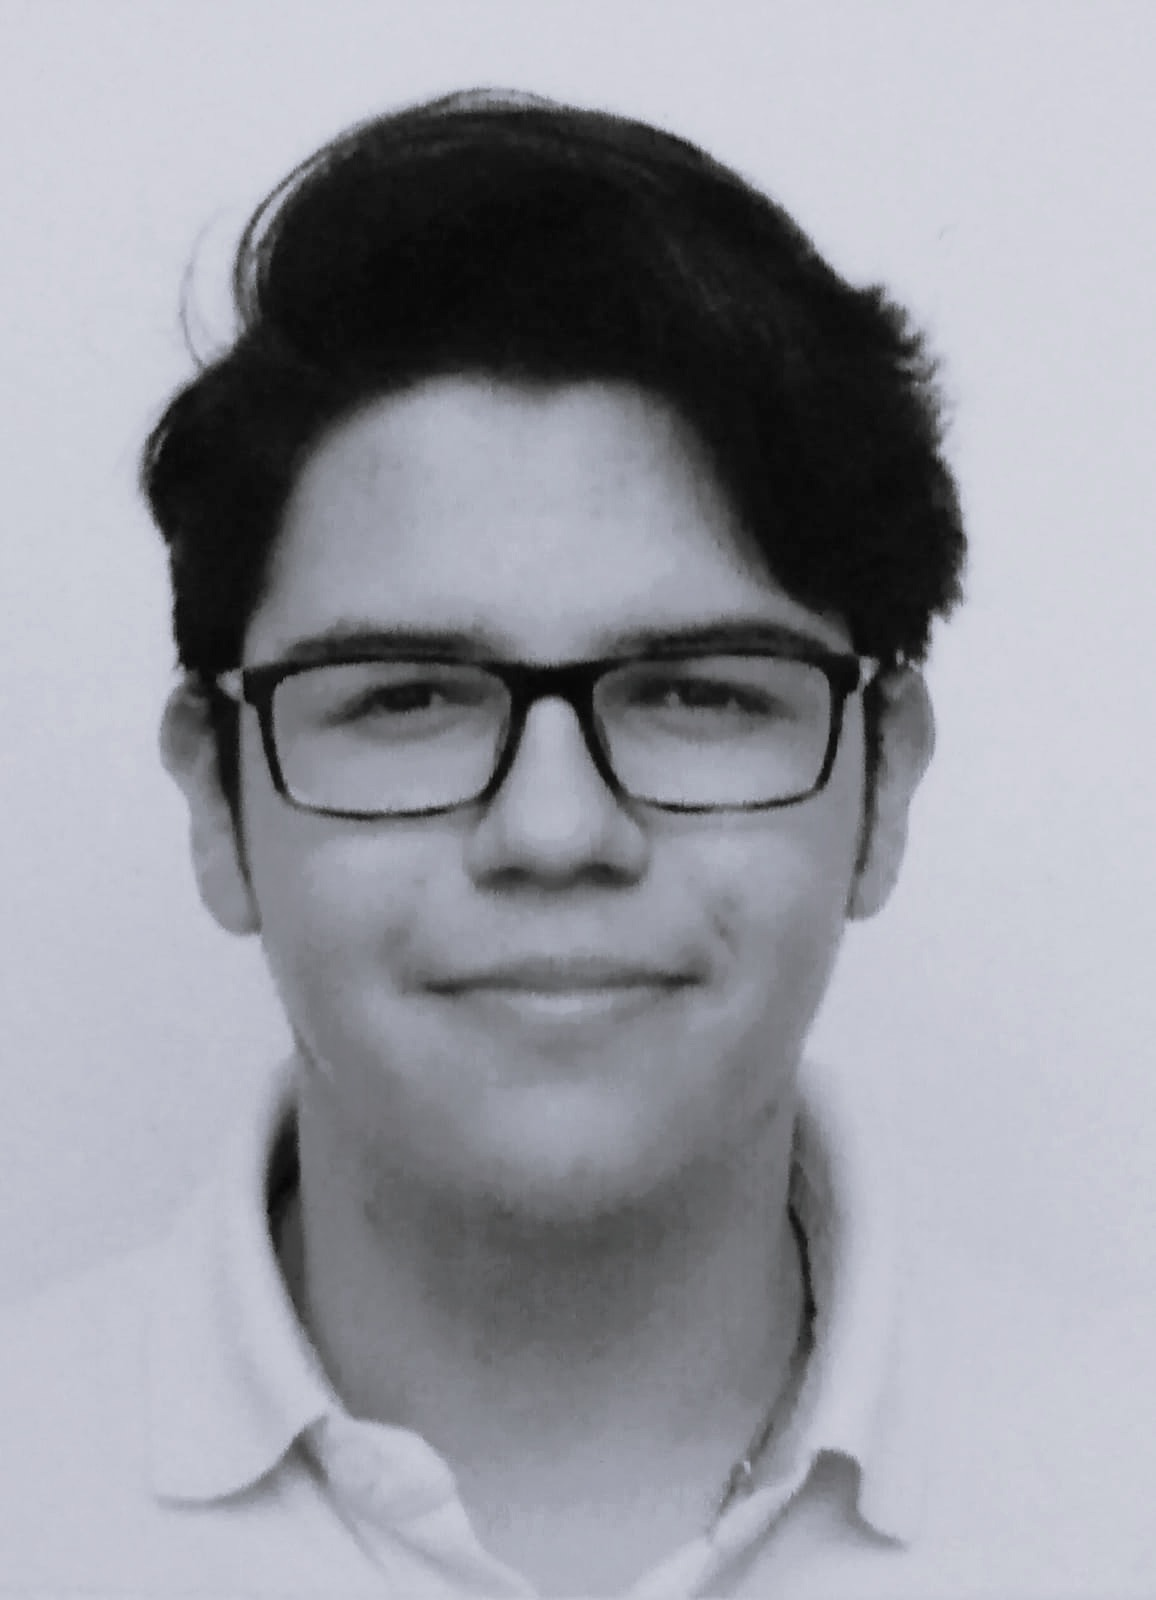
\includegraphics[width=1in,height=1.25in,clip,keepaspectratio]{nmv_bn}}]{Nicolás Mena-Valerio}
	Estudiante de Ingeniería Electrónica, Instituto Tecnológico de Costa Rica, desde 2022.
	Correo, nimena@estudiantec.cr
\end{IEEEbiography}

\begin{IEEEbiography}[{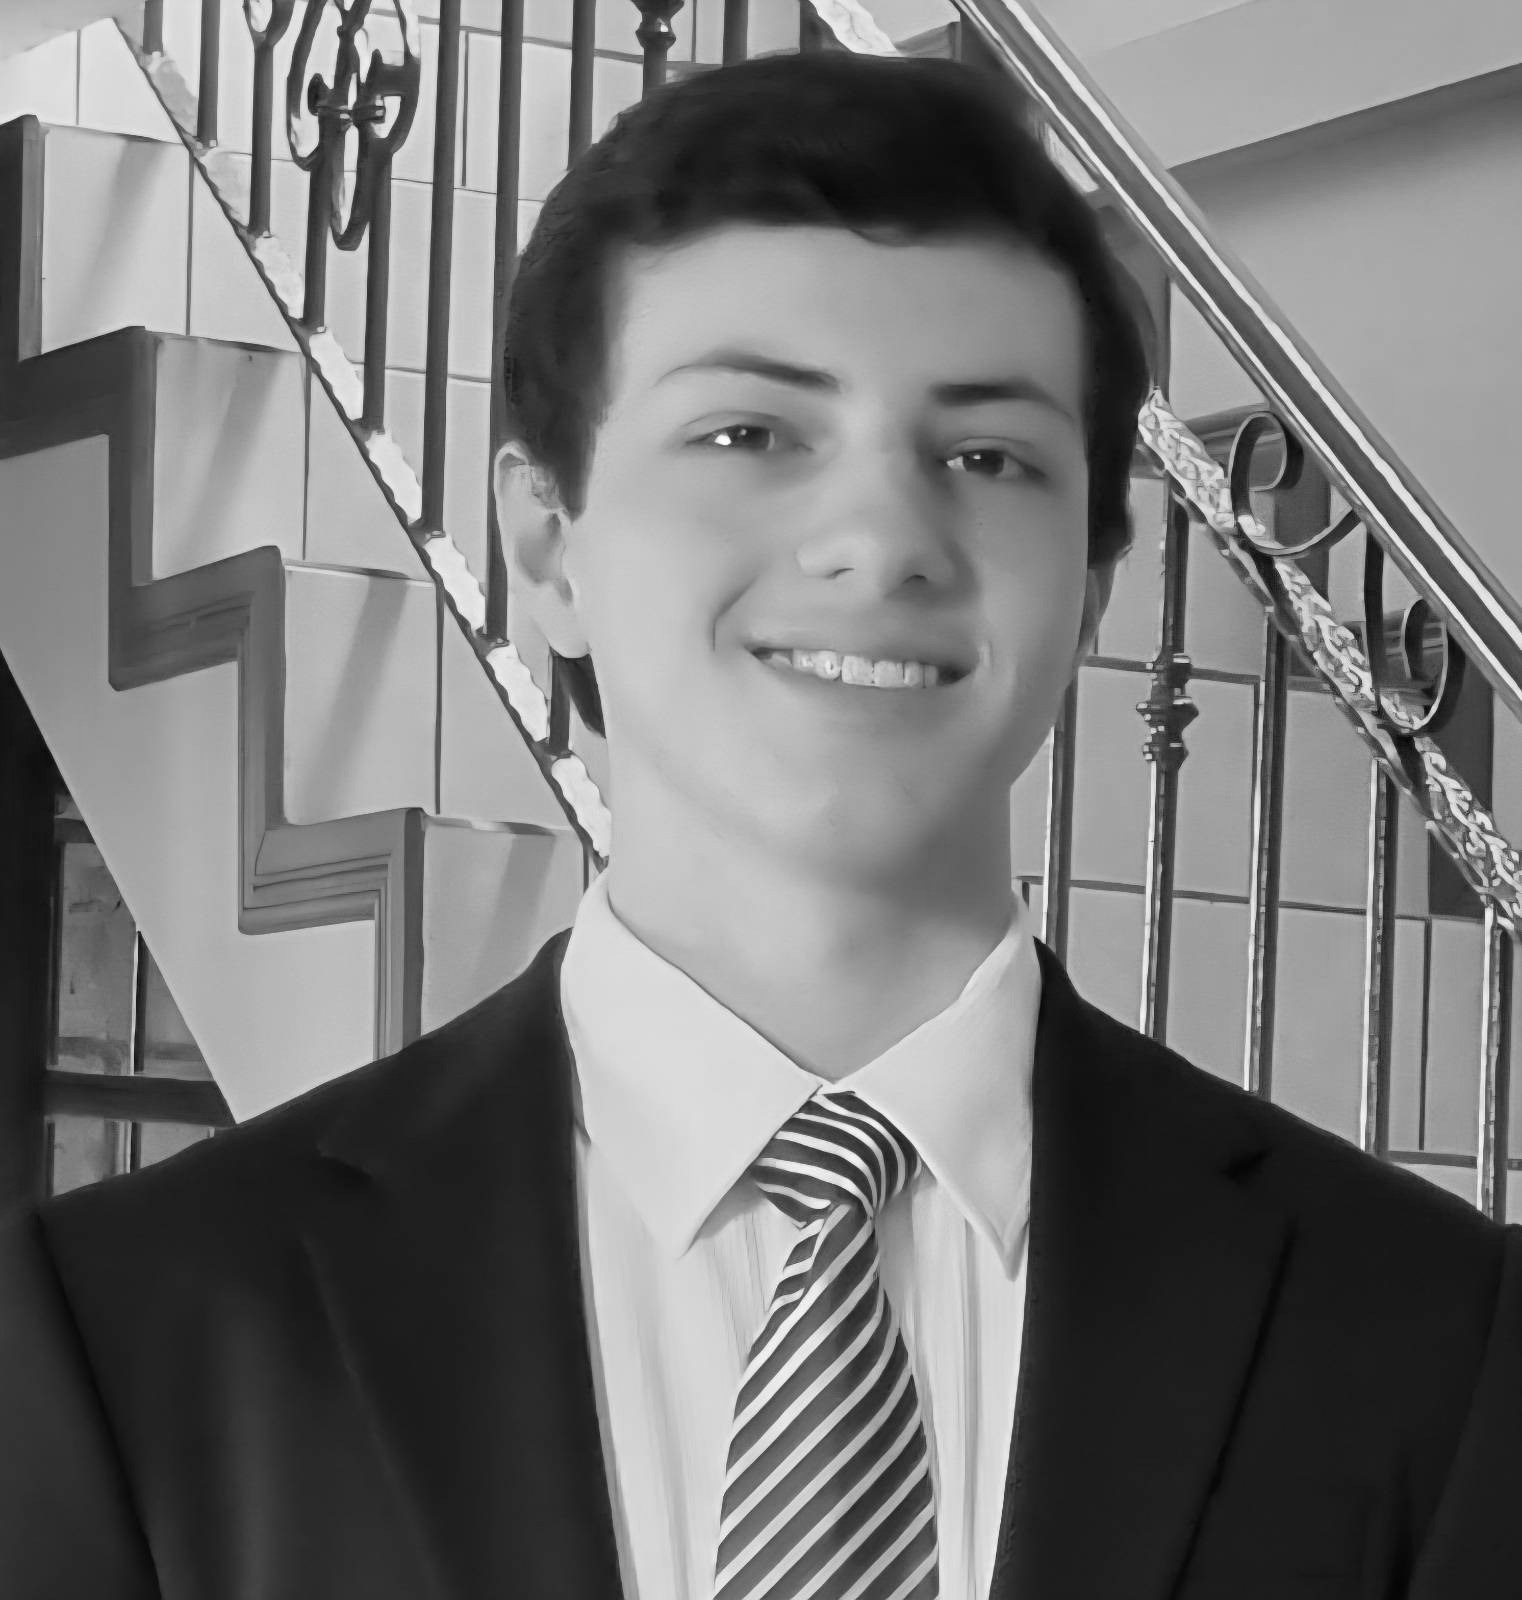
\includegraphics[width=1in,height=1.25in,clip,keepaspectratio]{mcq_bn}}]{Mattio Coghi-Quirós}
	Estudiante de Ingeniería Electrónica, Instituto Tecnológico de Costa Rica.
	Correo, mcoghi@estudiantec.cr
\end{IEEEbiography}

\vfill
\end{document}